% Copyright (c)  2005-2010 EDF-EADS-PHIMECA.
% Permission is granted to copy, distribute and/or modify this document
% under the terms of the GNU Free Documentation License, Version 1.2
% or any later version published by the Free Software Foundation;
% with no Invariant Sections, no Front-Cover Texts, and no Back-Cover
% Texts.  A copy of the license is included in the section entitled "GNU
% Free Documentation License".
\renewcommand{\etapemethodo}{B}
\renewcommand{\nomfichier}{docref_B11_EmpiricalCDF}
\renewcommand{\titrefiche}{Empirical cumulative distribution function}

\Header

\MathematicalDescription{

  \underline{\textbf{Goal}} \vspace{2mm}

  The empirical cumulative distribution function provides a graphical representation of the probability distribution of a random vector without implying any prior assumption concerning the form of this distribution. It concerns a non-parametric approach which enables the description of complex behaviour not necessarily detected with parametric approaches.

  Therefore, using general notation, this means that we are looking for an estimator $\widehat{F}_N$ for the cumulative distribution function $F_{X}$ of the random variable $\vect{X} = \left( X^1,\ldots,X^{n_X} \right)$:
  $$
  \widehat{F}_N \leftrightarrow F_{X}
  $$
  \vspace{2mm}

  \underline{\textbf{Principle of the method for $\boldsymbol{n_X = 1}$}} \vspace{2mm}

  Let us first consider the uni-dimensional case, and let us denote $\vect{X} = X^1 = X$. The empirical probability distribution is the distribution created from a sample of observed values $\left\{x_1, x_2, \ldots, x_N\right\}$. It corresponds to a discrete uniform distribution on $\left\{x_1, x_2, \ldots, x_N\right\}$: where $X'$ follows this distribution,
  $$
  \forall \; i \in \left\{1,\ldots, N\right\} ,\ \textrm{Pr}\left(X'=x_i\right) = \frac{1}{N}
  $$

  The empirical cumulative distribution function  $\widehat{F}_N$ with this distribution is constructed as follows:
  $$
  F_N(x) = \frac{1}{N} \sum_{i=1}^N \mathbf{1}_{ \left\{ x_i \leq x \right\} }
  $$

  The empirical cumulative distribution function $F_N(x)$ is defined as the proportion of observations that are less than (or equal to) $x$ and is thus an approximation of the cumulative distribution function $F_X(x)$ which is the probability that an observation is less than (or equal to) $x$.
  $$
  F_X(x) = \textrm{Pr} \left( X \leq x \right)
  $$

  The diagram below provides an illustration of an ordered sample $\left\{5,6,10,22,27\right\}$.
  \begin{center}
    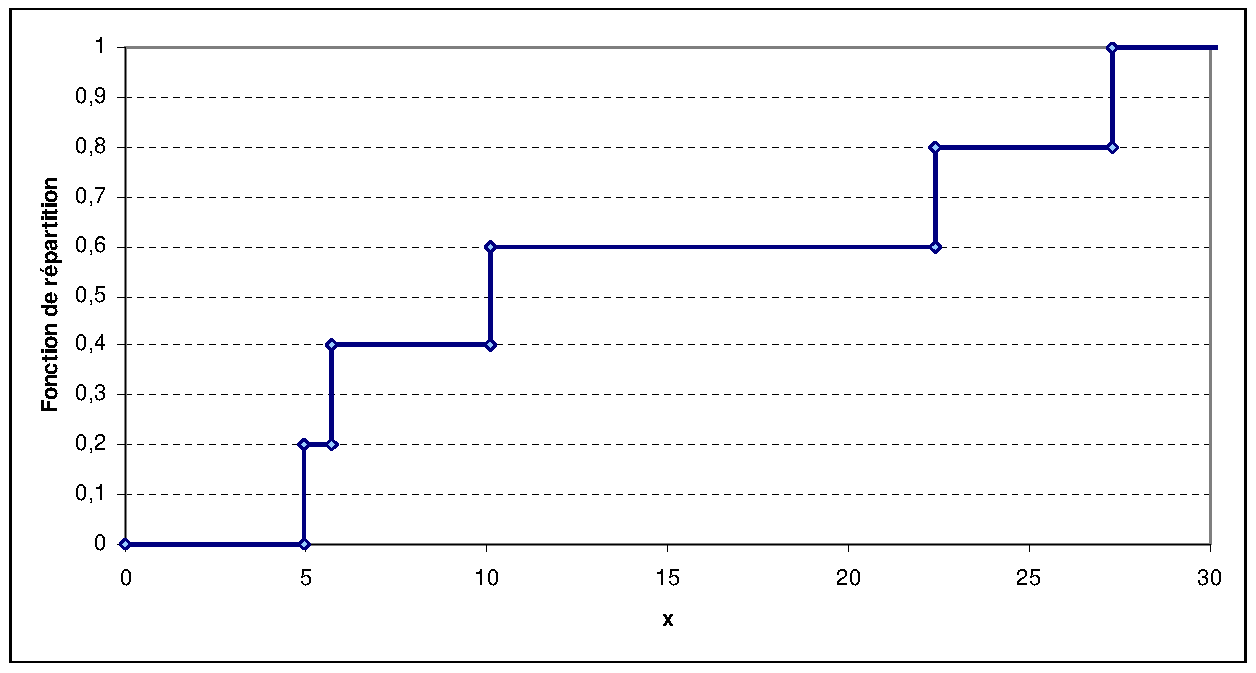
\includegraphics[scale=0.5]{foncrep.pdf}
  \end{center}
  \vspace{2mm}

  \underline{\textbf{Principle of the method for $\boldsymbol{n_X > 1}$}} \vspace{2mm}

  The method is similar for the case $n_X>1$. The empirical probability distribution is a distribution created from a sample $\left\{\vect{x}_1, \vect{x}_2, \ldots, \vect{x}_N\right\}$. It corresponds to a discrete uniform distribution on $\left\{\vect{x}_1, \vect{x}_2, \ldots, \vect{x}_N\right\}$~: where $\vect{X}'$ follows this distribution,
  $$
  \forall \; i \in \left\{1,\ldots, N\right\} ,\ \textrm{Pr}\left(\vect{X}'=\vect{x}_i\right) = \frac{1}{N}
  $$
  Thus we have:
  $$
  F_N(\vect{x}) = \frac{1}{N} \sum_{i=1}^N \mathbf{1}_{ \left\{ x^1_i \leq x^1,\ldots,x^{n_X}_N \leq x^{n_X} \right\} }
  $$
  in comparison with the theoretical probability density function $F_X$:
  $$
  F_X(x) = \Prob{X^1 \leq x^1,\ldots,X^{n_X} \leq x^{n_X}}
  $$
}
{
  This method is also referred to in the literature as the empirical distribution function.
}

\Methodology{
  This method is used in step B "Quantifying Sources of Uncertainty". It enables us to obtain a representation of the distribution of the vector $\vect{X}$ of uncertain variables defined in step A "Specifying Criteria and the Case Study", without applying any a priori modelling hypotheses.
}
{
  This method has the advantage of depending only on the observed values, without any other modelling assumptions (as in the \otref{docref_B11_KernelSmoothing}{kernel smoothing method}). Nevertheless, in the case where little data is available, the estimation of the criteria defined in step A can be less precise with this non-parametric method than with a parametric approach (e.g. the models described in \otref{docref_B121_DistributionSelection}{standard parametric models}).

  The following bibliographical references provide main starting points for further study of this method:
  \begin{itemize}
  \item Saporta G. (1990). "Probabilit�s, Analyse de donn�es et Statistique", Technip
  \item Dixon W.J. \& Massey F.J. (1983) "Introduction to statistical analysis (4th ed.)", McGraw-Hill
  \end{itemize}
}
